\section{Evidence II: arXiv's rules as experiments}\label{sec:causal}

The facts above are correlations. This section uses arXiv's own rules, which
create variation in how much a paper is read, in the cost of entering, in the
cost of catching up on a literature and in how much one person may write. The
data are the arXiv metadata snapshot of 18 October 2026 \citep{kaggle2026}:
2.2 million papers with new-style identifiers submitted from 2015 to 15
October 2026, with the exact time of each submission, the submitter's name,
the author list and the abstract. \Cref{app:data} documents every construction.
\Cref{tab:listing,tab:policies} report the estimates.

\paragraph{Reconstructing the daily listings.} arXiv announces new papers once a
day. Papers submitted before the daily cutoff appear in that evening's listing,
and later papers wait for the next one. Identifiers are assigned at announcement,
in listing order. Within an announcement batch, the rank correlation between
identifier and submission time is 0.98 for papers that were not held for
moderation (median across batches). Six percent of papers are held and announced
later. The submission-time distribution reveals the cutoff. It was 16:00
Eastern Time until the end of 2016 and has been 14:00 since January 2017. On an
average weekday about 15 papers are submitted in the first ten seconds after 14:00:00:
authors race for the top of the next listing \citep{haqueginsparg2009}. We
place every paper in its announcement batch and rank it within its primary
category's list of new submissions.

\subsection{Does reading protect? Listing position as a readership shock}

\Cref{lem:credit} gives sharp predictions for a shock that makes a paper $i$
more visible to the researchers who might later cover it. If visibility raises
the probability $\varphi$ that a later covering project detects $i$, unaware
duplicates of $i$ fall by $\theta\,\dd\varphi$, aware follow-ons that cite $i$
rise by $q\theta\,\dd\varphi$, and the ratio of the two effects identifies $q$,
the share of detections that proceed. We test these predictions with two
designs.

\paragraph{Design A: the daily cutoff.} A paper submitted just after 14:00 opens
the next listing, while one submitted just before closes the current one. The
first stage is sharp (\cref{tab:listing}, panel A; \cref{fig:listing}). Within an
hour of the cutoff, excluding a five-minute donut around the bunching, crossing
the cutoff raises the probability of being among the first five papers by
\empRDtopfive, from a base of \empRDtopfiveBefore. The comparison it delivers,
however, is first against \emph{last}. The end of a listing is also highly
visible, a ``reverse visibility'' effect documented for arXiv by
\citet{haqueginsparg2010} and for NBER working papers by
\citet{feenbergetal2017}. Submitters on the two sides also differ: those just
after the cutoff have fewer prior submissions (\empRDprior, SE \empRDpriorSE). Top-of-listing papers receive \emph{fewer} citations
than end-of-listing papers: \empRDcitesIns\ log points (SE \empRDcitesInsSE) in
high-energy physics, where INSPIRE-HEP gives complete citation counts, and
\empRDcitesSS\ (SE \empRDcitesSSSE) across all fields in the
\empRDcitesSSN\ papers with Semantic Scholar counts. The cutoff therefore does not isolate
visibility, and we do not use it to test detection.

\paragraph{Design B: rank within the listing.} A cleaner source of variation is
how many other papers happen to be submitted earlier on the same day. A
paper's position is one plus the number of papers in its category submitted
since the batch opened. We hold fixed the submission time (in 15-minute bins,
separately for the weekend batch), the category-year, the announcement date
and the size of the listing. Position then varies only with the timing of
other people's submissions. We use all \empRankN\ papers in the nine
categories covered by INSPIRE-HEP in 2017--2022, excluding the first 15 minutes
after the cutoff. The residual standard deviation of log position is
\empRankSD. Predetermined characteristics are balanced: number of authors and
the submitter's prior submissions are unrelated to residual position.
Abstracts are slightly shorter lower in the list (1.6 words of 151 per log point, SE 0.6).

The readership effect is small. One log point lower in the listing, roughly
moving from second to fifth place, reduces citations by \empRankCites\ log points
(SE \empRankCitesSE; \empRankCitesMain\ without date fixed effects). Position bins show
no premium for the very first slots once dates are held fixed. Later overlapping
work responds even less. We count later papers in the same category, within 24
months, by authors who do not overlap with the focal paper's, whose TF-IDF
similarity exceeds the category's median (75th percentile) of nearest-neighbour
similarity. With INSPIRE's curated reference lists we split them into those
that cite the focal paper (aware) and those that do not (unaware). One log point
lower in the listing changes unaware overlap at the 75th percentile threshold by
\empRankUsevfive\ (SE \empRankUsevfiveSE) on a mean of \empRankUsevfiveMean, and
aware overlap by \empRankAsevfive\ (SE \empRankAsevfiveSE). The 95\% interval
rules out an increase in unaware overlap of more than \empRankUsevfiveUB\ per log
point. The minimum detectable effect at 80\% power is \empRankUsevfiveMDE\ of the
mean. Self-follow-ups by the focal paper's own authors fall with position
(\empRankSelf, SE \empRankSelfSE). This suggests that attention encourages authors
to continue a line of work, or that the design leaves some day-level confounding;
either way it does not affect the comparison with other authors' work.

\paragraph{What this teaches.} Passive visibility moves casual readership a little
and does not move the detection of overlapping work. In the model, detection
depends on the coverage $R/P$ that a later researcher chooses and on search
precision $\sigma$, not on how prominently the earlier paper was announced. The
result says that the protective job of reading is done by targeted search when a
project is planned or written up, not by browsing daily listings. This matches
the high calibrated search precision needed for a 60\% aware share
(Fact~\ref{fact:aware}). The right causal test of $\varphi$ is therefore a
shock to the cost of search. \Cref{sec:predictions} sets out one: the blocking
of Google in mainland China from 2014 \citep{zhengwang2020}. The model predicts
that it lowered the aware share and raised unaware duplication in work by
China-based authors, relative to Hong Kong-based and overseas Chinese authors
in the same topics.

\begin{figure}[t]
\centering
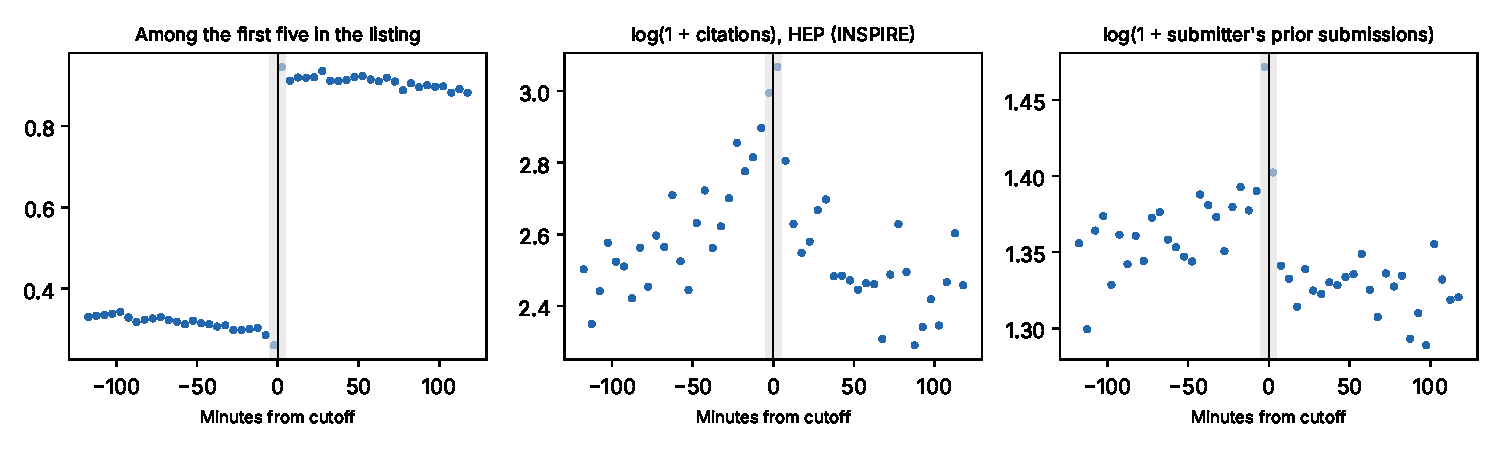
\includegraphics[width=\textwidth]{figures/emp_rd_listing.pdf}
\caption{The daily cutoff. Binned means, net of category-year means, by minutes
from the 14:00 ET cutoff (weekday submissions 2017--2022; shaded: five-minute
donut). Left: probability of being among the first five papers of the
category's listing. Middle: log citations in high-energy physics (INSPIRE-HEP).
Right: the submitter's prior submissions, a predetermined characteristic that
jumps at the cutoff. Papers just after the cutoff open the next listing; papers
just before close the current one.}
\label{fig:listing}
\end{figure}

\begin{table}[p]
\centering\footnotesize
\caption{Listing position, readership and later overlapping work}\label{tab:listing}
\begin{tabular}{@{}lrrrl@{}}
\toprule
Outcome & Estimate & (SE) & Mean & $N$ \\
\midrule
\multicolumn{5}{@{}l}{\emph{A. Discontinuity at the daily cutoff: submitted just after (top of next listing) vs.\ just before (end of current listing)}} \\
Position in listing (0 = top, 1 = bottom) & $-0.838$ & $(0.004)$ & 0.884 & 77,051 \\
Among the first five papers & $+0.688$ & $(0.006)$ & 0.300 & 77,051 \\
Number of authors (balance) & $-0.178$ & $(0.454)$ & 5.650 & 77,051 \\
Abstract length, words (balance) & $-0.832$ & $(0.917)$ & 153.785 & 77,051 \\
log(1 + submitter's prior submissions) (balance) & $-0.051$ & $(0.017)$ & 1.363 & 77,050 \\
log(1 + citations), HEP (INSPIRE) & $-0.137$ & $(0.060)$ & 2.682 & 11,483 \\
log(1 + citations), all fields (Semantic Scholar) & $-0.175$ & $(0.032)$ & 2.522 & 43,097 \\
\midrule
\multicolumn{5}{@{}l}{\emph{B. Listing rank in high-energy physics: effect of log position, holding submission time fixed}} \\
log(1 + citations) & $-0.023$ & $(0.016)$ & 2.309 & 87,679 \\
Citation percentile in category-year & $-0.005$ & $(0.003)$ & 0.480 & 87,679 \\
Later overlapping papers by others, $\tau_{50}$ & $-0.021$ & $(0.018)$ & 0.667 & 87,694 \\
\quad of which cite the focal paper (aware) & $-0.003$ & $(0.008)$ & 0.211 & 87,694 \\
\quad of which do not (unaware) & $-0.018$ & $(0.014)$ & 0.454 & 87,694 \\
Later overlapping papers by others, $\tau_{75}$ & $-0.005$ & $(0.006)$ & 0.130 & 87,694 \\
\quad aware & $-0.000$ & $(0.004)$ & 0.062 & 87,694 \\
\quad unaware & $-0.005$ & $(0.004)$ & 0.068 & 87,694 \\
Later overlapping papers by the same authors, $\tau_{50}$ & $-0.048$ & $(0.015)$ & 0.687 & 87,694 \\
\bottomrule
\end{tabular}

\par\smallskip
\begin{minipage}{\textwidth}\footnotesize
Notes: Panel A: local linear regression discontinuity at the 14:00 ET cutoff,
bandwidth 60 minutes, triangular kernel, donut of 5 minutes, separate slopes,
category-year and weekday fixed effects; standard errors clustered by
submission day; ``Mean'' is the mean just before the cutoff. Panel B: all
papers in hep-th, hep-ph, hep-ex, hep-lat, gr-qc, nucl-th, nucl-ex, astro-ph.CO
and astro-ph.HE announced in their regular batch, 2017--2022, submitted at least
15 minutes after the batch opened; regressors are log listing position and log
list size; fixed effects for category-year, submission-time bin (15 minutes;
hourly for the weekend batch) and announcement date; standard errors clustered by
announcement date. Overlap thresholds $\tau_q$ are percentiles of the
category's nearest-neighbour similarity distribution. Citations and reference
lists from INSPIRE-HEP (excluding self-citations) unless noted.
\end{minipage}
\end{table}

\subsection{Entry cost: the endorsement rule}

New arXiv submitters need an endorsement. Until late 2025, an e-mail address at
a recognised institution sufficed. On 10 December 2025 arXiv stopped accepting
it alone in Mathematics \citep{arxivendorsemath2025}, and on 21 January 2026 in
all sections \citep{arxivendorse2026}. New authors now need prior authorship of
an accepted paper in the section or a personal endorsement. We measure the share
of papers whose submitter has never submitted before. We compare each week with
the same week of the previous academic year, which removes seasonality, and
Mathematics with other sections, which exploits the staggered timing.

The first stage is large and well timed (\cref{tab:policies}, panel A;
\cref{fig:policies}). Net of the year before, the first-time submitter share fell by
\empEndMath\ percentage points in Mathematics (SE \empEndMathSE; about
\empEndMathRel\ of its base) and by \empEndOther\ points in other sections (SE
\empEndOtherSE; about \empEndOtherRel). In the six weeks when only Mathematics was
treated, Mathematics fell \empEndStag\ points more than the other sections (SE
\empEndStagSE). Submitters with no prior arXiv authorship, the group the rule
targets, fell by about \empEndNoTrackOtherRel\ outside Mathematics. In the model,
this is a rise in the cost of entering science. \Cref{prop:ai}(ii) predicts that
it reduces the number of topics roughly in proportion to the entrants it
removes, while leaving density, the overlap rate and the aware share nearly
unchanged, because $\mathcal E$ is small. Those outcomes need a year of
post-period data; \cref{sec:predictions} states them in advance.

\subsection{Catch-up cost: review articles in computer science}

Review articles summarise a literature and lower the cost of catching up on it
\citep{mcmahanmcfarland2021}. On 31 October 2025, arXiv began to require that
review and position papers in computer science be accepted after peer review
before posting \citep{arxivcsreview2025}. The share of computer-science papers
with review-type titles fell from \empCSpre\% to \empCSpost\%, from about
\empCSperMonthPre\ to \empCSperMonthPost\ a month. Relative to other archives the
fall is \empCSdid\ percentage points (SE \empCSdidSE), and it survives a CS-specific trend.
Reviews did not migrate to other primary categories cross-listed to computer
science (\cref{tab:policies}, panel B). Within computer science, categories that
had relied more on reviews lost more of them. A category with a 1 point higher
pre-period review share lost \empCSdoseFS\ points more (SE \empCSdoseFSSE),
against an insignificant placebo a year earlier.

In the model, fewer reviews mean slower catch-up, a higher $\kappa$ and
therefore lower mature density, more topics and fewer overshooting topics
(\cref{prop:ai}(iv)). The short-run implication is less entry into existing
topics where reviews mattered. The share of papers with a first-time author fell
more in review-reliant categories: \empCSdoseRF\ per unit of exposure (SE
\empCSdoseRFSE). The same regression a year earlier gives \empCSdoseRFpl\ (SE
\empCSdoseRFplSE), so part of the gradient predates the rule. We read the reduced
form as suggestive. The topic-level predictions are stated in
\cref{sec:predictions}.

\subsection{A cap on writing: two submissions per person per month}

On 1 October 2026, arXiv limited every submitter to two new submissions per
calendar month, without prior announcement and with no exemptions
\citep{arxivratelimit2026}. The cap applies to the submitting account, not to the
authors. Because shared names belong to different people, we measure excess
submissions among names whose submissions in a half-month fall in a single
archive. In the first half of each month of 2026 before the cap, \empCapPre\ of
papers were a submitter's third or later submission; in October the share was
\empCapOct, a residual consistent with shared names and proceedings accounts. The
cap therefore removed about \empCapRemoved\ of papers mechanically. Volume did not
fall. Papers per weekday rose \empCapVol\ log points from the first half of
September to the first half of October 2026, against \empCapVolPrev\ on average in
2024--2025. Categories more exposed to heavy submitters did not grow less
(\cref{tab:policies}, panel C). Per-submitter caps bind on a sliver of output
and can be met by letting a co-author submit. In the model's terms, the cap
is not a shock to writing speed, and the model predicts that a binding one,
being a policy inside topics, would be largely dissipated by entry.

\subsection{Drafting speed: author-level adoption of LLM-style writing}

\Cref{prop:ai}(i) predicts that faster drafting raises papers per researcher one
for one. To measure drafting at the author level, we follow the
excess-vocabulary literature \citep{liangetal2024,kobaketal2025}. We flag
abstracts that use words whose frequency jumped after ChatGPT (``delve'',
``showcase'', ``underscore'', ``intricate'', ``pivotal'', and similar). Their share
rose from 3\% of abstracts in 2022 to 11\% in 2024. Among \empLLMn\ submitters
active in 2021--2022 and 2023, the \empLLMadopters\ who used such words in at
least half of their 2023 abstracts are adopters. Submitters who never used them
are the comparison group. Classification uses 2023 papers only, so the outcome
window, 2024--2026, is not conditioned on it. With submitter and field-by-half-year
fixed effects, adopters' log(1 + papers per half-year) rose by \empLLMall\ (SE
\empLLMallSE), about \empLLMallPct\ more papers, and by \empLLMnonai\ (SE
\empLLMnonaiSE) in fields where AI is not the subject (\cref{fig:llm} in
\cref{app:data}). Pre-period coefficients drift by up to \empLLMpre, so part of
this is a pre-existing trend. The drafting channel is present but small:
adopters have so far used language models to write differently more than to
write more.

\begin{figure}[t]
\centering
\begin{subfigure}{0.49\textwidth}
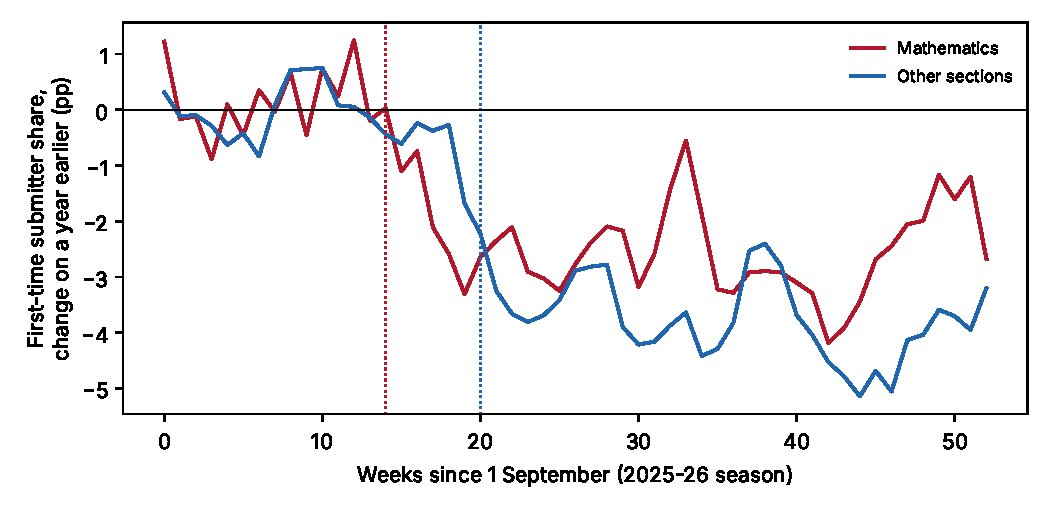
\includegraphics[width=\textwidth]{figures/emp_endorsement.pdf}
\caption{Endorsement rule}
\end{subfigure}\hfill
\begin{subfigure}{0.49\textwidth}
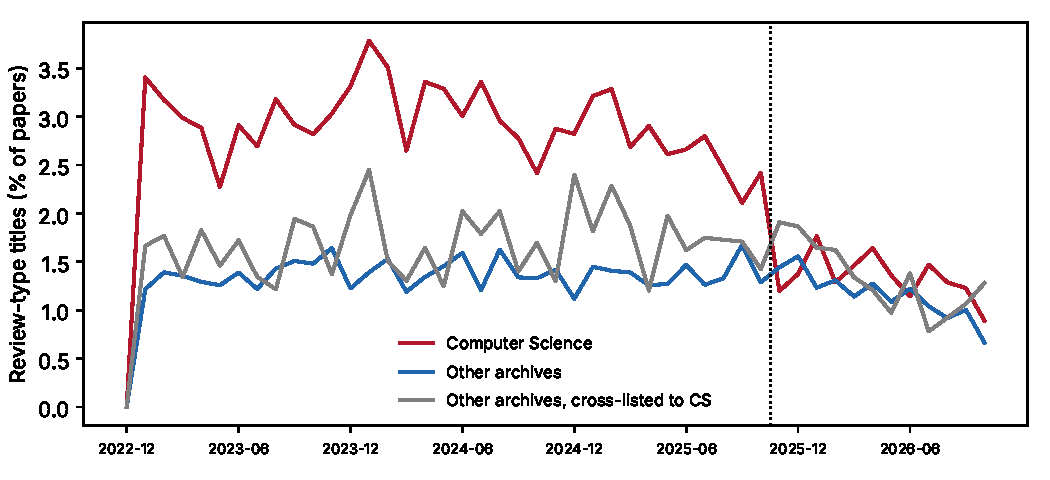
\includegraphics[width=\textwidth]{figures/emp_cs_reviews.pdf}
\caption{CS review policy}
\end{subfigure}
\caption{Two arXiv rule changes. (a) First-time submitter share, change on the same
week a year earlier (three-week moving average), Mathematics and other sections;
dotted lines mark 10 December 2025 and 21 January 2026. (b) Share of papers with
review-type titles by archive; the dotted line marks November 2025.}
\label{fig:policies}
\end{figure}

\begin{table}[p]
\centering\footnotesize
\caption{arXiv rule changes as shocks to entry, catch-up and writing}\label{tab:policies}
\resizebox{\textwidth}{!}{\begin{tabular}{@{}lrrl@{}}
\toprule
Design and outcome & Estimate & (SE) & Pre-period mean \\
\midrule
\multicolumn{4}{@{}l}{\emph{A. Endorsement tightening (entry cost): Mathematics 10 Dec 2025, all sections 21 Jan 2026}} \\
First-time submitter share, Mathematics, vs.\ year before & $-0.024$ & $(0.003)$ & 0.141 \\
First-time submitter share, other sections, vs.\ year before & $-0.034$ & $(0.003)$ & 0.222 \\
First-time submitter share, Mathematics vs.\ others, 10 Dec--20 Jan & $-0.017$ & $(0.004)$ & \\
Submitters with no prior arXiv authorship, Mathematics & $-0.009$ & $(0.003)$ & 0.043 \\
Submitters with no prior arXiv authorship, other sections & $-0.009$ & $(0.002)$ & 0.054 \\
log number of first-time submitters, other sections & $-0.154$ & $(0.035)$ & \\
\midrule
\multicolumn{4}{@{}l}{\emph{B. Peer review required for CS review and position papers (catch-up cost), 31 Oct 2025}} \\
Review-type share of papers, CS vs.\ other archives & $-0.013$ & $(0.001)$ & 0.027 \\
\quad with a CS-specific linear trend & $-0.010$ & $(0.002)$ & \\
\quad leakage: non-CS primary cross-listed to CS & $-0.002$ & $(0.001)$ & \\
Within CS: change in review share on pre-period review share & $-0.41$ & $(0.10)$ & 0.027 \\
\quad placebo, one year earlier & $-0.13$ & $(0.09)$ & \\
Within CS: change in first-time-author share on review share & $-0.70$ & $(0.26)$ & \\
\quad placebo, one year earlier & $-0.32$ & $(0.17)$ & \\
\midrule
\multicolumn{4}{@{}l}{\emph{C. Two submissions per submitter per month (writing cap), 1 Oct 2026}} \\
Third-or-later submissions in days 1--15, single-field names: Jan--Sep 2026 & $1.66\%$ & & \\
\quad October 2026 (residual: shared names and proceedings accounts) & $0.38\%$ & & \\
log papers per weekday, Oct 1--15 vs.\ Sep 1--15: 2026 & $+0.220$ & & \\
\quad same change in 2024 and 2025 & $+0.173$, $+0.178$ & & \\
Category dose-response: change on exposure (vs.\ 2025) & $+0.03$ & $(2.95)$ & 0.016 \\
\midrule
\multicolumn{4}{@{}l}{\emph{D. Author-level adoption of LLM-style writing (drafting speed)}} \\
log(1 + papers per half-year), adopters vs.\ others, 2024--26, all fields & $+0.022$ & $(0.005)$ & 0.48 \\
\quad fields where AI is not the subject (no cs, stat, eess) & $+0.024$ & $(0.007)$ & 0.52 \\
\bottomrule
\end{tabular}
}
\par\smallskip
\begin{minipage}{\textwidth}\footnotesize
Notes: Panel A: weekly cells by announcement week, September 2024--October 2026;
each week is differenced against the same week a year earlier; Newey--West
standard errors (four lags). Panel B: monthly cells, 2023--2026, archive and month
fixed effects, robust standard errors; dose-response across 29 CS categories with
at least 300 papers a year, weighted by size, Nov--Oct years. Panel C: days 1--15
of each month, papers announced in their regular batch; exposure is the
category's Jan--Sep 2026 share of excess submissions. Panel D: submitter and
field-by-half-year fixed effects, standard errors clustered by submitter.
Identities are name keys throughout (\cref{app:data}).
\end{minipage}
\end{table}

\subsection{What the shocks say about the model}

The four designs do not test every proposition, and two of them are first
stages whose outcomes are still accruing. Together they establish three
things. The entry margin responds to its cost, which is what makes density
respond little to volume. The supply of review articles, a lever on catch-up
costs, responds to policy, and the first reduced form on entry has the sign the
model predicts. And the detection of overlapping work does not run through
passive visibility. Reading protects through deliberate search, which is why
better search tools, not more prominent announcements, are the channel through
which AI could move the aware share. A per-person writing cap, finally, is not a
lever on volume at all.
